\documentclass[conference]{IEEEtran}
\usepackage{graphicx}
\usepackage{float}
\usepackage{amsmath}
\usepackage{hyperref}
 \hypersetup{
     colorlinks=true,
     linkcolor=blue,
     filecolor=blue,
     citecolor = black,      
     urlcolor=blue,
 }

% Add space between paragraphs
% skip 12pt
% indent 12pt
\usepackage[skip=\baselineskip, indent=\baselineskip]{parskip}

% Code and pseudocode style
\usepackage{listings}
\lstset{
    frame=tb, % draw a frame at the top and bottom of the code block
    numbers=left, % display line numbers on the left
    xleftmargin=5.0ex, % adjust leftmargin
    breaklines, %add breaklines if overfull \hbox
    tabsize=2,
    inputencoding = utf8,  % Input encoding
    extendedchars = true,  % Extended ASCII
    literate      =        % Add support for accents in Listings
      {á}{{\'a}}1  {é}{{\'e}}1  {í}{{\'i}}1 {ó}{{\'o}}1  {ú}{{\'u}}1
      {Á}{{\'A}}1  {É}{{\'E}}1  {Í}{{\'I}}1 {Ó}{{\'O}}1  {Ú}{{\'U}}1
      {à}{{\`a}}1  {è}{{\`e}}1  {ì}{{\`i}}1 {ò}{{\`o}}1  {ù}{{\`u}}1
      {À}{{\`A}}1  {È}{{\'E}}1  {Ì}{{\`I}}1 {Ò}{{\`O}}1  {Ù}{{\`U}}1
      {ä}{{\"a}}1  {ë}{{\"e}}1  {ï}{{\"i}}1 {ö}{{\"o}}1  {ü}{{\"u}}1
      {Ä}{{\"A}}1  {Ë}{{\"E}}1  {Ï}{{\"I}}1 {Ö}{{\"O}}1  {Ü}{{\"U}}1
      {â}{{\^a}}1  {ê}{{\^e}}1  {î}{{\^i}}1 {ô}{{\^o}}1  {û}{{\^u}}1
      {Â}{{\^A}}1  {Ê}{{\^E}}1  {Î}{{\^I}}1 {Ô}{{\^O}}1  {Û}{{\^U}}1
      {œ}{{\oe}}1  {Œ}{{\OE}}1  {æ}{{\ae}}1 {Æ}{{\AE}}1  {ß}{{\ss}}1
      {ç}{{\c c}}1 {Ç}{{\c C}}1 {ø}{{\o}}1  {Ø}{{\O}}1   {å}{{\r a}}1
      {Å}{{\r A}}1 {ã}{{\~a}}1  {õ}{{\~o}}1 {Ã}{{\~A}}1  {Õ}{{\~O}}1
      {ñ}{{\~n}}1  {Ñ}{{\~N}}1  {¿}{{?`}}1  {¡}{{!`}}1
      {°}{{\textdegree}}1 {º}{{\textordmasculine}}1 {ª}{{\textordfeminine}}1
      % ¿ and ¡ are not correctly displayed if inconsolata font is used
      % together with the lstlisting environment. Consider typing code in
      % external files and using \lstinputlisting to display them instead.      
}

\renewcommand\IEEEkeywordsname{Keywords}

\makeatletter
\def\endthebibliography{%
  \def\@noitemerr{\@latex@warning{Empty `thebibliography' environment}}%
  \endlist
}
\makeatother

\hyphenation{op-tical net-works semi-conduc-tor}

%%%%%%%%%%%%%%%%%%%%%%%%%%%%%%%%%%%%%%%%%%%%%%%%%%

\begin{document}

\nocite{*}

\title{Behavioral Biometrics: User Authentication using Keystroke Dynamics}

\author{\IEEEauthorblockN{Berrospi Rodriguez, Luis Alfonso}
\IEEEauthorblockA{Computer Science\\
Universidad de Ingeniería y Tecnología\\
Lima, Perú\\
luis.berrospi@utec.edu.pe}
}

\maketitle

\begin{IEEEkeywords}
Behavioral biometrics, keystroke dynamics, machine learning, user authentication, cybersecurity, deep learning, CNN, RNN, GRU.
\end{IEEEkeywords}

\begin{abstract}

    Keystroke dynamics, a biometric authentication technique, has gained significant attention due to its potential for secure user identification and verification. This paper presents a comprehensive review of the type of text used in keystroke dynamics, the features extracted from the data, and the classification algorithms used. Then two algorithms are proposed, one based on metric distance to compare data with a nearest neighbor algorithm and another based on a hybrid neural network architecture that use a CNN and a RNN. The algorithms where tested with public datasets from Universities. The results, according to the literature, are an Equal Error Rate (EER) of 8.4\% for the nearest neighbor algorithm and 5.97\% for the hybrid neural network.
\end{abstract}

\IEEEpeerreviewmaketitle

\section{Introduction}

Since the start of the digital age, cybersecurity has been developing and adapting to the new threats that arise in the digital world. One of the topics of great importance in this field is user authentication. Different methods have been used over the years, such as passwords, iris recognition, fingerprint matching, etc. However, most of these methods seek to guarantee the authentication only at the beginning of the session of interaction between a human and a device, but not through said session. This creates a problem: if a user leaves their already authenticated session open, anyone can access their information. For this reason, the use of behavioral biometrics has been proposed. These authentication methods allows the user to be authenticated not only at the beginning of the session but also throughout it \cite{behavior}.

Keystroke Dynamics are behavioral biometrics that provides the authentication a user at the beginning and throughout a session by analyzing the patterns and rhythm that they present when writing using a keyboard \cite{combine_distance}. This techniques were suggested during World War II \cite{secondworldwar} when the idea of using the rhythm of the Morse code to identify the operator of a telegraph was proposed. But it was not until the develop of computers and the Internet studies started to encourage the use of this technique \cite{monrose2000keystroke}.


The main problem with the Keystroke Dynamics techniques as a method for user authentication is the different algorithms, data extraction methods and features used to authenticate a user. Different comparison techniques have been used through the years. Probabilistic methods \cite{bleha1990login}, multiple machine learning techniques \cite{machine_learning} and Neural Networks are some examples of these techniques \cite{pnn, deep_learning}. All these techniques have very different results, some of the best achieve an average FAR of 2\% while others are between 8 and 27\% \cite{typing_patterns}. In addition, it has been shown that precision can vary depending on what is being written. It has been possible to observe how the precision goes from 79\% with text that is transcribed to 21\% with text that is freely written \cite{old} and how if a person is writing in a particular context, like programmers writing code, the algorithms can reach a precision of 98.6\% \cite{programmers}.

The goal of this document is to implement two algorithms for user authentication through Keystroke Dynamics that have already been proposed in the literature. It is seeked to compare the results obtained by each of the algorithms, and determine which of them is the most appropriate for this type of authentication. In addition, this project also pursue to determine the behavior of each algorithm with respect to the type of data that is used, this is, if the algorithm is more accurate with free text or with fixed text.

\section{Theoretical Foundations}

In the following section, the theoretical foundations of keystroke dynamics are going to be explained. First, the type of texts that can be used for the feature extraction phase is going to be explained. Then, the features that are going to be extracted from the text are going to introduced. Finally, the different algorithms that are going to be used are going to be explained along with some characteristics of biometric systems that can be used to evaluate the performance of each algorithm.

\subsection{Data extraction}

It is possible to define two types of text that can be used for feature extraction:

\begin{itemize}
	\item Fixed text: This type of text is the one that is written by the user using a fixed source. It is generally a short phrase or a word that is used to identify the user. A good example of this type of text is the password and username that are employed to log into a computer or a website.

	\item Free text: This type of text is the one that is written by the user without any restriction. This kind of text is the most common in the real world but it is generally the most difficult to analyze because of the lack of restrictions and the introduction of important factors like, the user's level of concentration, thinking time, etc.
\end{itemize}



\subsection{Features}

In general, the features extracted from the keystroke dynamics are based on the study and analyzes data involving digraphs and trigraphs. In the keystroke dynamics literature a digraph is a set of two consecutive characters that represents two keystrokes, that can be letters, numbers or symbols and other keys that do not necessarily represent a language character like the space bar, shift key or enter key. Logically, a trigraph is a set of three consecutive characters that represents three keystrokes \cite{trigraphs}. Some of the most common features that can be extracted from a single keystroke, a digraphs or a trigraphs are the following \cite{monrose2000keystroke, machine_learning}:

\begin{itemize}
	\item Tap timestamp: Defined as the timestamp of the key press.
	\item Release timestamp: Defined as the timestamp of the key release.
	\item Time between keystrokes: This feature is commonly defined as the time that elapses between the key press of the first keystroke and the key release of the second keystroke of a digraph or trigraph.
	\item Hold time: This is defined as the time that elapses between the key press and the key release of a keystroke.
	\item Words per minute (WPM): This is the average number of words that a user can type in a minute.
	\item Percentage of usage of special keys: This feature is defined as the percentage of times that a user uses keys like the shift key or Caps-Lock key.
\end{itemize}

\subsection{Classification techniques}

Once the features are extracted, the next step is to use algorithms to authenticate the user. Most of these techniques can be classified into two groups.


The first group is based on the usage of distance metrics. These set of techniques are take use of the calculation of the distance between the features of the user that is trying to be identified and the features of the users that are already registered in the system. Features are displayed as a vector of multiple dimensions and the distance between vectors is calculated using a distance metric. Some metrics that can be used are the Manhattan distance and the Mahalanobis distance.

On one hand, Manhattan distance for $n$ dimensions can be defined as the sum of the absolute differences between the coordinates of the vectors, As represented in the following formula:

\begin{equation}
	d(x,y) = \sum_{i=1}^{n} |x_i - y_i|
\end{equation}

Where $x$ and $y$ are vectors of $n$ dimensions and $x_i$ and $y_i$ are the $i$th coordinates of the vectors $x$ and $y$ respectively.

On the other hand Mahalanobis distance can be defined as the distance between two points that depends on the probability distribution of all the points \cite{de2000mahalanobis}. The squared version of this distance can be described by the following formula:

\begin{equation}
	d(x,y) = (x-y)^T S^{-1} (x-y)
\end{equation}

Where $x$ and $y$ are vectors of $n$ dimensions and $S$ is the covariance matrix of the set of points.


These distances are commonly used in clustering algorithms like K-nearest neighbors. This algorithm stores the multidimensional feature vectors such that when a vector is received it can be classified by the majority of the classes of the nearest neighbors using a distance metric. In the user authentication problem, the user can be identified by finding the single nearest neighbor and using a threshold to determine if the user is the same as the one that is trying to be identified. A simple knn example for 2 dimensional features can be shown in figure \ref{fig:knn}.

\begin{figure}[h]
    \centering
    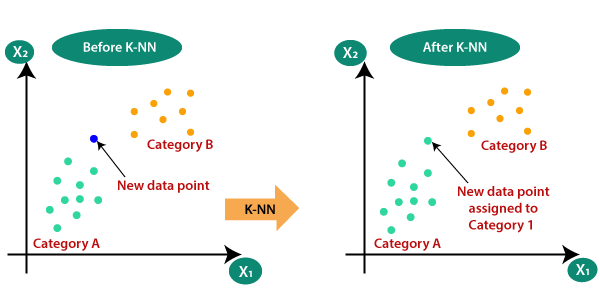
\includegraphics[width=0.7\linewidth]{images/knn}
    \caption{K-nearest neighbors algorithm \cite{knn}}
    \label{fig:knn}
\end{figure}

The second group of techniques is based on the use of deep learning techniques.

One of the most important parts of this approach is the use of algorithms to vectorize the text, such that said text can be used as input for the neural network. Some of the most common vectorization techniques try to represent text as numbers, assigning numeric values to words, characters or more complex structures like tokens. Other techniques try to transform images into matrices that contain RGB or grayscale values of the pixels. Finally there are techniques that have numbers as input and try to normalize and standardize the data to perform better in the neural network.

This techniques are characterized by the use of neural networks. These networks try to simulate the human brain by being composed of multiple layers of neurons that are connected to each other. Each neuron is a mathematical function that receives multiple inputs and produces one or more outputs.

The neural networks that are going to be used in this project are the following:

\begin{itemize}
	\item Convolutional Neural Networks: CNNs are a type of neural network architecture that have been successful in tasks such as image classification, object detection, image segmentation, by feature extraction. \cite{valueva2020cnn}. They are designed to automatically learn and extract hierarchical patterns and features from input data. CNNs use convolutional layers, pooling layers, and fully connected layers \cite{taye2023layers}. Convolutional layers apply filters to the input data, capturing spatial dependencies and detecting local patterns. Pooling layers reduce the spatial dimensions of the data. Fully connected layers are usually placed at the end of the network and are used to get the final output.
	\item Recurrent Neural Network: RNNs are neural network architectures suitable for sequential data such as time series, text, and speech\cite{li2015rnn_structure}. Unlike traditional networks, RNNs contain loops that allow information to persist and be processed across different time steps \cite{dupond2019rnn}. The presence of a hidden state, the internal memory of the network, grants RNNs the ability to capture temporal dependencies and contextual information within the data.
	\item Gated Recurrent Unit: GRU is a variation of RNN designed to address the vanishing gradient problem and improve the modeling of long-term dependencies. GRU incorporates gatelike mechanisms that regulate the flow of information within the network. GRU units consist of an update gate and a reset gate, which control the operations of information update and reset in the hidden state \cite{cho2014gru}. The update gate determines how much of the previous hidden state to retain, while the reset gate decides how much of the previous state to forget. GRUs have demonstrated superior performance over traditional RNNs in various tasks such as language modeling, machine translation, and speech recognition \cite{ravanelli2018gruperformance}.
\end{itemize}

\subsection{benchmark}

The following factors are used to evaluate the performance of biometric systems \cite{benchmarks}:

\begin{itemize}
	\item False Acceptance Rate (FAR):
	FAR is a metric used in biometric system benchmarking to measure the likelihood of the system incorrectly granting access to unauthorized individuals. It represents the rate at which the system mistakenly identifies impostors as genuine users. A lower FAR indicates a higher level of security, as it means the system is less likely to mistakenly accept unauthorized individuals. This characteristic can be represented by the following formula:

	\begin{equation}
		FAR = \frac{\text{False Acceptances}}{\text{Total Impostor Attempts}}
	\end{equation}
	
	\item False Rejection Rate (FRR):
	FRR is a metric used to assess the probability of the biometric system incorrectly rejecting legitimate users. It represents the rate at which the system fails to recognize or authenticate genuine users. A lower FRR indicates better user convenience, as it means the system is less likely to deny access to legitimate users. This metric can be represented by the following formula:
	\begin{equation}
		FRR = \frac{\text{False Rejections}}{\text{Total Genuine Attempts}}
	\end{equation}
	
	\item Equal Error Rate (EER):
	EER is a benchmark point where the FAR and FRR are equal as seen in Figure \ref{fig:eer}. It signifies the threshold or decision boundary at which the system achieves a balance between false acceptances and false rejections. The EER provides a summary measure of the system's performance and is commonly used for comparing different biometric systems. A lower EER indicates better overall performance, as it reflects a balanced trade-off between security and user convenience.
	\begin{figure}[h]
	    \centering
	    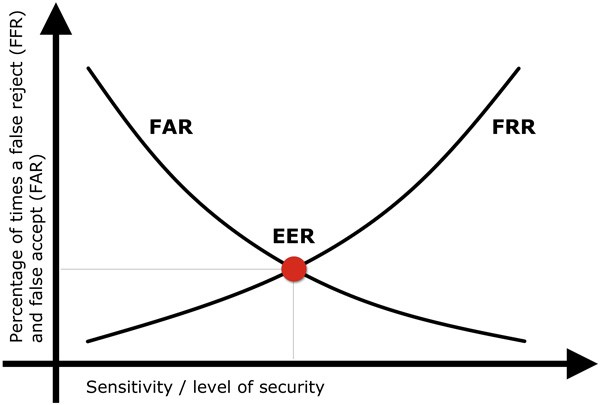
\includegraphics[width=0.7\linewidth]{images/eer}
	    \caption{Equal Error Rate \cite{eer}}
	    \label{fig:eer}
	\end{figure}
\end{itemize}

\section{Related Work}

Multiple approaches have been proposed to solve the problem of user authentication through keystroke dynamics. It is possible to classify said approaches into two main categories: those that focus on what data is obtained and those that focus on the classification algorithm. In the first category, work have been done comparing and analyzing results with free text and transcribed text \cite{old,programmers} and with memorized text like usernames and passwords \cite{bleha1990login, pnn}. In the second category, work have been done using different classification algorithms, such as distance metrics \cite{combine_distance}, multiple machine learning techniques \cite{machine_learning} and Neural Networks \cite{deep_learning, maiorana2019deepkey}.

Previous work has shown that in some cases simple distance based clustering algorithms can accomplish good performance \cite{robinson1998login, bergadano2002norm_distance,de2000mahalanobis,programmers} this have been explained by the fact that the there are some distances that handle effectively characteristics of the features present in keystroke dynamics, like the correlations  and good interaction between the features. Some examples of these distances are Mahalanobis which takes into account the covariance matrix of the features for better differentiation and  Manhattan distance which is more robust, it is not affected by the scale of the features \cite{combine_distance}. 

It also have been shown that the selection of the features is a key factor for the performance of the models and that the algorithms used for the classification are less important \cite{pnn}. This can be seen in the continuous integration of new features throughout the development of the techniques. At the beginning, the data was obtained from the time between 2 keystrokes  \cite{bleha1990login} and then the pressing time was added \cite{robinson1998login}. Later more sophisticated features were added like the edit time \cite{machine_learning}, normalized data so that the emotional state of the user does not affect the results  and the introduction of trigraphs \cite{bergadano2002norm_distance}.

In recent years the use of deep learning techniques has been studied and proposed to solve the problem of user biometric recognition through keystroke dynamics. A hybrid model involving a CNN and a RNN was proposed in \cite{deep_learning} using feature transformation to adapt the input data to a image-like format for better results. More simple models have also been proposed \cite{maiorana2019deepkey}, using CNN an fixing the input size with a 6 digit pin on mobile devices.

\section{Techniques}

In this section, we describe the 2 techniques that are going to be implemented in this project. The first one proposed by Yu Zhong et al \cite{combine_distance}, which use a common technique with distance metrics for user authentication. The second one is the technique proposed by Lu, Xiaofeng, et al \cite{deep_learning}, which uses a hybrid model of a CNN and a RNN.

\subsection{Distance Metrics}

The first technique proposed by Yu Zhong et al \cite{combine_distance} is based on the use of distance metrics to compare the data of a user with the data of the rest of the users. The data used in this technique comes from the CMU Keystroke Dynamics Benchmark and it is made up by the time between keystrokes and the hold time of each keystroke. This dataset contains 51 users, each one with 400 samples (feature vectors) of a fixed password written in English.

After a state of the art analysis, the authors realized that the 2 more successful distance metrics used in the literature were the Manhattan distance and the Mahalanobis distance. So they decided to combine them in a new distance metric so that the new metric could take advantage of the benefits of both. The new metric is defined as follows:

Firstly, the authors apply the following linear transform to the data like the Mahalanobis distance, so that the features become uncorrelated with equal variations.
\begin{equation}
	x' = \Phi x
\end{equation}
Where $\Phi$ is the principle of the square root of the covariance matrix $S$ of the data such that $S^{-1} = \Phi \cdot \Phi^T$.

Then the Manhattan distance is measured between the transformed data.
\begin{equation}
	d(x',y') = \sum_{i=1}^{n} |x_i' - y_i'|
\end{equation}

Then, the authors apply the Manhattan distance to the transformed data. Finally, this new distance is used to compare the data of a user with the other data with a standard Nearest Neighbor classifier.

The authors also used an outlayer detection technique in the training of the model to improve the results. This technique is based on the use of the median $\mu$ and the standard deviation $\sigma$ of the features so that only the feature vectors with  its $i$th feature in the range $[\mu_i - k\sigma_i, \mu_i + k\sigma_i]$ are used in the training of the model.

This technique achieved an EER of 8.4\% This result improved the results previously obtained \cite{killourhy2009comparing} of the Manhattan distance (EER of 9.6\%) and the Mahalanobis distance (EER of 10\%).

\subsection{Deep Learning}

The authors of \cite{deep_learning} propose a hybrid model of a CNN and a RNN to identify the user. The model is based on the use of a CNN to extract the features from the keystroke dynamics and a RNN to identify the user. The model used the Clarkson II and Buffalo datasets for keystroke dynamics. These datasets contained the timestamp of each keystroke, recollected from 103 user in the Clarkson II dataset and 157 in the Buffalo dataset. Booth of this datasets contained free text written by the users, but the Clarkson II dataset also contained data from the users writing a fixed text.

First, the data had to be vectorized. The vector data format was defined by the authors as can be seen in the following table \ref{tab:deep_learning_vector_data_format}.

\begin{table}[H]
	\centering
	\begin{tabular}{|c|c|c|c|c|c|}
		\hline
		ID{[}1{]} & ID{[}2{]} & H{[}1{]} & H{[}2{]} & D{[}1{]}H{[}2{]} & D{[}1{]}D{[}2{]} \\ \hline
	\end{tabular}
	\caption{Vector data format proposed by the authors of \cite{deep_learning}}
	\label{tab:deep_learning_vector_data_format}
\end{table}

Where D[$n$] is the timestamp of the $n$th keystroke tap, H[$n$] is the hold time of the $n$th keystroke and ID[$n$] is the key identifier of the $n$th keystroke keystroke, U[$n$] reefers to the timestamp of the $n$th key release. In addition, D[$n$]U[$m$] is the UD characteristic of the $n$th and the $m$ keys and D[$n$]D[$m$] is the DD characteristic of the $n$th and the $m$ keys.

Following this format, a vector of 6 features can be created from text. As can be shown in the image \ref{fig:deep_learning_vector_data_format}.

\begin{figure}[H]
	\centering
	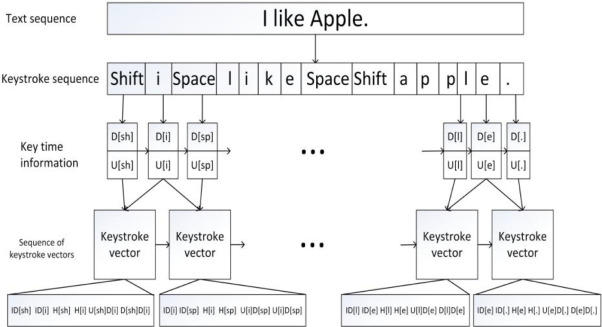
\includegraphics[width=0.5\textwidth]{images/vectorization.jpg}
	\caption{Vector data format transform by the authors of \cite{deep_learning}}
	\label{fig:deep_learning_vector_data_format}
\end{figure}

Then, the authors proposed multiple configurations of the neural network architecture. However, the more effective can be see in the image \ref{fig:deep_learning_architecture}.

\begin{figure}[H]
	\centering
	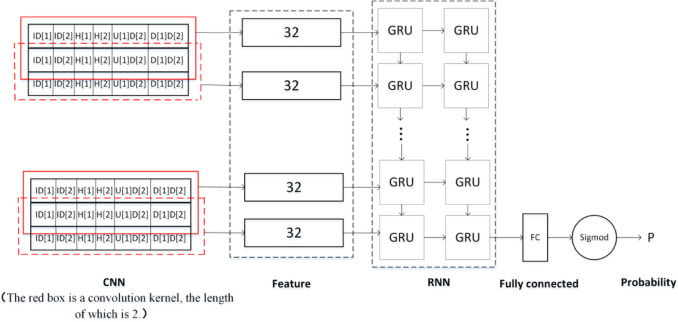
\includegraphics[width=0.5\textwidth]{images/architecture.jpg}
	\caption{Neural network architecture proposed by the authors of \cite{deep_learning}}
	\label{fig:deep_learning_architecture}
\end{figure}

As it can be seen, all the vectors extracted from a given text with specific length in terms of keystrokes are arrange as a matrix where each row is a vector. Then, a one dimensional CNN with a convolutional kernel with length 2 (feature vectors) is applied to the matrix to extract 32 the features that are going to be used by the RNN, a double layer GRU. Finally, the output of the RNN connected to the fully-connected layer and then to the output layer, which is a sigmoid function that outputs the probability of the user being the user that the model is trying to identify. The authors also added dropout layers to each layer of the model to avoid overfitting.

This approach obtained a FRR of 2.07\%, a FAR of 3.26\% and an EER of 2.67\% using the Clarkson II dataset and a FRR of 6.61\%, a FAR of 5.31\% and an EER of 5.97\% using the Buffalo dataset.

\section{Experiments}

\subsection{Comparison metrics}

Biometric systems have transformed the landscape of identity verification and access control, offering a reliable and efficient way to authenticate individuals based on their unique physical or behavioral traits. These systems leverage characteristics like fingerprints, iris patterns, voiceprints, facial features, or gait patterns to establish an individual's identity. However, even with their advancements, biometric systems are not immune to errors and uncertainties. Therefore, it becomes essential to evaluate their performance using well-defined metrics.

The evaluation of biometric systems involves analyzing various aspects of their performance, including accuracy, reliability, and security. Among the key metrics used for this purpose are the False Acceptance Rate (FAR), False Rejection Rate (FRR), and Equal Error Rate (EER). These metrics provide valuable insights into the system's ability to correctly identify and authenticate individuals while managing the delicate balance between accepting impostors (false acceptance) and rejecting legitimate users (false rejection).

The False Acceptance Rate (FAR) signifies the probability of the system mistakenly accepting an impostor or granting access to an unauthorized individual. Conversely, the False Rejection Rate (FRR) reflects the likelihood of the system erroneously rejecting a legitimate user. Both FAR and FRR play crucial roles in assessing system performance, as they directly impact the security and usability of biometric systems.

The Equal Error Rate (EER) is another vital metric that offers a balanced evaluation of system performance. It represents the threshold at which the FAR and FRR intersect, indicating the point where the rates of false acceptance and false rejection are equal. EER serves as a benchmark for comparing different biometric systems, enabling system administrators to select an optimal threshold that balances security and usability considerations.

A comprehensive understanding of FAR, FRR, and EER is essential in evaluating the performance of biometric systems. By quantifying the rates of false acceptance and false rejection, these metrics facilitate the identification of vulnerabilities, system limitations, and areas for improvement. Additionally, they contribute to the establishment of standards, benchmarks, and best practices for deploying reliable and efficient biometric authentication systems.

In this monograph, we explore the definitions, calculation methods, and significance of FAR, FRR, and EER in biometric systems. We delve into the trade-off between FAR and FRR, discussing the factors that influence their values. Furthermore, we examine the role of EER as a balanced evaluation metric and its importance in system selection and performance benchmarking.

By gaining insights into these metrics, researchers, practitioners, and decision-makers can make informed choices regarding the design, implementation, and enhancement of biometric systems. Additionally, a deeper understanding of FAR, FRR, and EER empowers stakeholders to evaluate the effectiveness, reliability, and security of biometric technologies in real-world applications.



\bibliographystyle{IEEEtran}
\bibliography{references}


\end{document}

anonfiles.com/t6bdn8fcy4/1_mp4
anonfiles.com/v8b5n4f8y8/Sin_t_tulo_png
anonfiles.com/z0b7n3f4y3/vlcsnap-2018-12-19-03h28m50s549_png
anonfiles.com/3fb4naf9y4/2_mp4
anonfiles.com/54b5n9fey2/vlcsnap-2019-01-27-23h45m08s578_png
anonfiles.com/reb0n7f6yf/1.mp4_jpg
anonfiles.com/74b2nef8yb/vlcsnap-2018-12-19-02h12m58s022_png
anonfiles.com/98b7n0f8ye/vlcsnap-2019-01-27-23h44m59s244_png